\documentclass[twocolumn,floatfix,nofootinbib,aps]{revtex4-1}
\usepackage[utf8]{inputenc}

\usepackage{amsmath}    % need for subequations
\usepackage{amssymb}    % for symbols
\usepackage{graphicx}   % need for figures
\usepackage{verbatim}   % useful for program listings
\usepackage{color}      % use if color is used in text
\usepackage{subfigure}  % use for side-by-side figures
%\usepackage{hyperref}   % use for hypertext links, including those to external documents and URLs
\usepackage[capitalise]{cleveref}   % use for referencing figures/equations
\begin{document}

\title{Opt-K}
\author{Robert T. McGibbon}
\author{Christian R. Schwantes}
\author{Vijay S. Pande}
\maketitle


Likelihood framework for choosing the optimal number of states in a
Markov State Model

\section{Overview}

A significant challenge in the automated construction of markov state
models is choosing the number of microstates. The number of microstates,
$k$ governs a bias-variance tradeoff -- when $k$ is large, the models
have a lot of parameters enabling it to fit the data with low bias, but
the simultaneous estimation of these parameters from finite data can
lead to high variance. On the other hand, when $k$ is small, we have
fewer parameters and better statistics, but at the expense of model
flexibility.

Currently, most MSM construction pipelines involve manually selecting
the number of states. This is done primarily by human intuition, and is
a significant bottleneck.

Here, we introduce a likelihood framework enabling the automatic
selection of the number of states.

Within the discrete state space, the likelihood of an ensemble of
trajectories given the MSM is straightforward. We simply take the
product of the state to state transition probabilities along the path.
These state to state transition probabilities are our main central
parameters, the entries of the transition matrix. However, as we vary
the number of states, it is not permissible to simply compare these
likelihoods to select an optimal number of states. Doing so, we would
always chose the trivial model, with only one state, as the transition
probability in that model would be $1$ and thus the likelihood of any
trajectory within that state space would be $1$.

The proper likelihood is not of the trajectory within the discrete state
space; instead it's the likelihood of the trajectory within the
continuous phase space, on which the discrete states are merely an
indicator function basis. 

\begin{equation}
P[X_{0...T-1}] dx^T = \prod_{i=0}^{T-1} T(X_i \rightarrow X_{i+1}) \cdot \prod_{i=0}^{T} p(X_{i} | \sigma(X_{i}))
\label{eq:like}
\end{equation}

With a discrete, non-overlapping state space, the likelihood of the
trajectory can be decomposed into a product over the trajectory of two
types of terms: the state to state transition probabilities and the
``emission'' probabilities of each state, the probability of observing a
conformation at a given location in phase space given that the
conformation ($x_t$) is within a certain state ($\sigma(x_t)$).

\section{Emission Distributions}

Up until this point, the emission probability distributions have not
been a model parameter for MSMs. Nevertheless, they are a critical
parameter from the point of view of evaluating trajectory likelihoods.
For example, consider two MSMs with the same transition probabilities.
However, in one case, the emission distributions for each state are
highly peaked at specific locations in phase space, whereas in the other
model the emission distributions are uniform over the volume of the
clusters. If the trajectory actually does go through the regions of high
likelihood in the first model, we would say that the first model more
accurately fits the data.

However, the long timescale behavior of the MSM, the quantity of most
interest scientifically, is independent of the choice of the emission
distributions. It's only determined by the eigenspectrum of the
transition matrix elements. (The emission distributions determine the
estimated eigenfunctions, but not the eigenvectors.)

Therefore, the most appropriate emission distribution for discrete state
MSMs is that of the uniform distribution over the phase-space volume of
the state. That is, the likelihood of observing a conformation in phase
space given that the conformation is assigned to state $i$ is $0$
if the conformation is outside of the bounding volume of the state and
constant if the conformation is within the volume. The constant is set
so that the distribution integrates to $1$, and is thus the reciprocal
volume of the microstate.

% \begin{align*}
% p(x | s) &= C \\
% \int p(x | s) dx &= 1 \\
% \int C \mathbf{1}_s dx &= 1 \\
% C &= \frac{1}{\int \mathbf{1}_s dx}
% \end{align*}

\begin{equation}
\label{eq:like_vol}
P[x_{0...T-1}] dx^N = \prod_{i=0}^{T-1} T(x_i \rightarrow x_{i+1}) \cdot \prod_{i=0}^T \frac{1}{V_{\sigma(x_{i})}}
\end{equation}

\section{Algorithm}

To use this uniform distribution emission model, computationally, we
need to compute the volume of our MSM states, which are high-dimensional
Voronoi cells. While trivial in two or three dimensions, this
computational geometry task becomes challenging in large dimensional
settings. The computation of high dimensional volumes has occupied significant
attention in recent years in the computational geometry literature, especially
via randomized algorithms. [See issue \#1 on the github]

One challenge is how to model the volume of states which are at the
``edge'' of the model. Is the volume of these states unbounded, given that they extend all the way out to infinity in some direction? This would be problematic.
It seems appropriate to assert that the volume of these edge states is bounded in some way by the extent of our dataset. For example, the volume of a state might be defined as the volume of the intersection of its Voronoi cell and the convex hull of the whole dataset.

We use a slightly modified version of this definition that adopts
the same spirit. Instead of taking the outer bounding region to be the convex hull of the data, we take it to be the set of all trial points such that the nearest data point to the trial point is closer than a certain cutoff, $R$. This can be computed relatively efficiently using a BallTree data structure. For further efficiency, we might use only a random subsample of the dataset for this nearest neighbor computation.

Instead of computing the volume of the Voronoi cells explicitly, we instead
compute the ratio of volume of each Voronoi cell to the volume of the entire
bounding region. Because the bounding region's volume is independent of the clustering parameters, its inclusion changes all of the calculated likelihoods by a constant multiplicative factor, and can thus be discarded from the perspective of model comparison.

To compute the fractional volumes of the Voronoi cells, we use the following randomized algorithm. First, we generate points inside of the bounding region using the lazy random walk Markov chain Monte Carlo algorithm.\cite{Kannan97} This random walk converges to sampling from the uniform distribution over the interior. After a sufficient burn in period, for each sampled point we compute its nearest MSM state center, assigning it to that state. As the number of randomly sampled points goes to infinity, the fraction of the points assigned to each state converges to being proportional to the state's volume.

This algorithm is highly amenable to parallel computation. For a euclidean
distance metric, the assignment can be performed efficiently by using a BallTree 
data structure for fast neighbor search.

\section{Choosing the Optimal Number of States}

We choose both the clustering algorithm (k-centers, k-means, etc) and the
number of states by maximizing the BIC/AIC scores of the model, using this
likelihood.

Unfortunately, this doesn't really help with picking the projection operator
to vectorize the conformations (e.g. dihedrals, contact maps, etc). Also,
it's not going to work rigorously with RMSD.

\section{Validation}

\subsection{Langevin Dynamics on the M\"uller Potential}
We being by using the procedure described above on data generated by simulating Langevin dynamics on the M\"{u}ller potential (\cref{fig:muller_pot}). This data was clustered into models of different sizes using one of two algorithms. The first, K-Centers, tends to make equal sized states as it works to minimize the maximum distance between a conformation and its generator. The second, Hybrid, will make varying size states because it works to minimize the average distance between conformations and their generators. In both cases, we built models ranging from 50 to 1,000 total states. Since this space is only two-dimensional, we used the simple, brute-force MC algorithm for calculating volumes. 

Briefly, we generated uniform random vectors within a bounding box whose size was slightly larger than the data. This random sample was then accepted if it was 'close enough' to a generator in the 100 state model, where close enough meant it was within 0.2 units from any generator in that model. This was used to approximate the convex hull of the data. Then the accepted points were assigned to a state. Then the volume of a state is proportional to the number of samples assigned to that state divided by the total number of samples. We note, that these volumes are actually in units of the total acceptable volume. This affects the absolute value of the likelihood, however, since the total volume was constant in all cases, the relative likelihoods are the same.
\begin{figure}[h!]
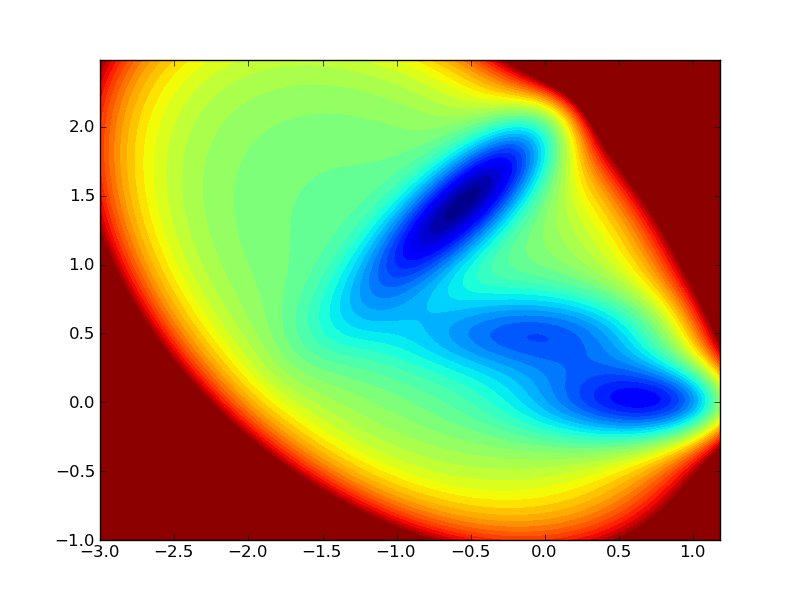
\includegraphics[width=2in]{figs/muller_pot.png}
\caption{The M\"{u}ller potential consists of three metastable wells. We simulated Langevin dynamics on this potential as a validation of the new likelihood function.}
\label{fig:muller_pot}
\end{figure} 

We built an MSM using a fixed lag time for each state decomposition and then calculated the likelihood according to \cref{eq:like_vol}. These likelihoods increased rapidly with $k$, but then plateaued at a value of around 300 states \cref{fig:like_kcenters}. At this plateau, we can conclude that we do not gain any new information by adding new states to our model and so should pick $k$ to be this point. This is a heuristic argument that can be made more mathematically rigorous with the introduction of functions like the Bayesian Information Content (BIC), which is defined in \cref{eq:bic}.

\begin{equation}
BIC = -2 \log L + m \log(n) 
\label{eq:bic}
\end{equation} Here, $L$ denotes the likelihood of a model, while $m$ is the number of parameters used in the model, and $n$ is the number of data points. Essentially this is a mathematical way of saying we would like to use a model with the maximum likelihood, but without introducing too many parameters. 
% don't know how to say this yet:
%We note that we cannot take this too seriously, and there are many other such criteria, such as the Aikaike Information Content (AIC). %%%
We found that the BIC of the models built using K-Centers clustering has a minimum at $k=250$. This minimum is the ``optimal'' model according to the BIC of our likelihood. As a check of the usefulness of this minimum, we plotted the three slowest implied timescales in the models as a function of $k$. The optimal model was close to the point at which the implied timescales became constant. 

\begin{figure}
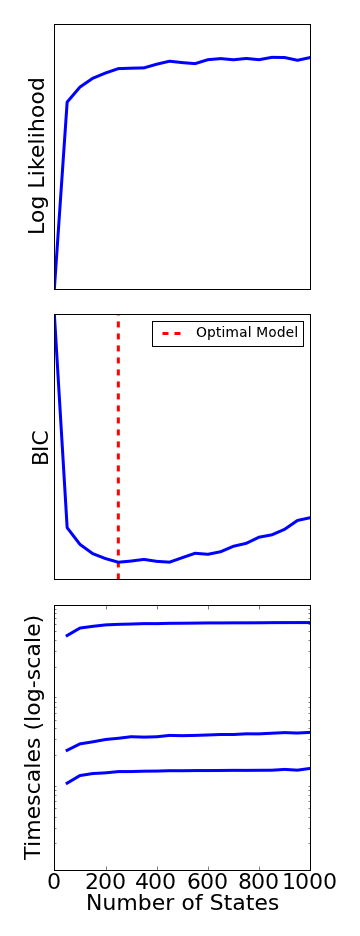
\includegraphics[width=2in]{figs/like_comp.png}
\caption{For models built between 50 and 1,000 states using the K-Centers algorithm, the log likelihood function increased quickly and plateaued at approximately 300 states. Heuristically, at this point, adding another state does not add anything to the model. As a result, by using a criterion, like the BIC, that penalizes using additional parameters to fit the data, we can find an ``optimal'' model. Interestingly, the BIC optimal model occurs at 250 states, which also corresponds to where the three slowest timescales plateau.}
\label{fig:like_kcenters}
\end{figure}

\begin{figure*}
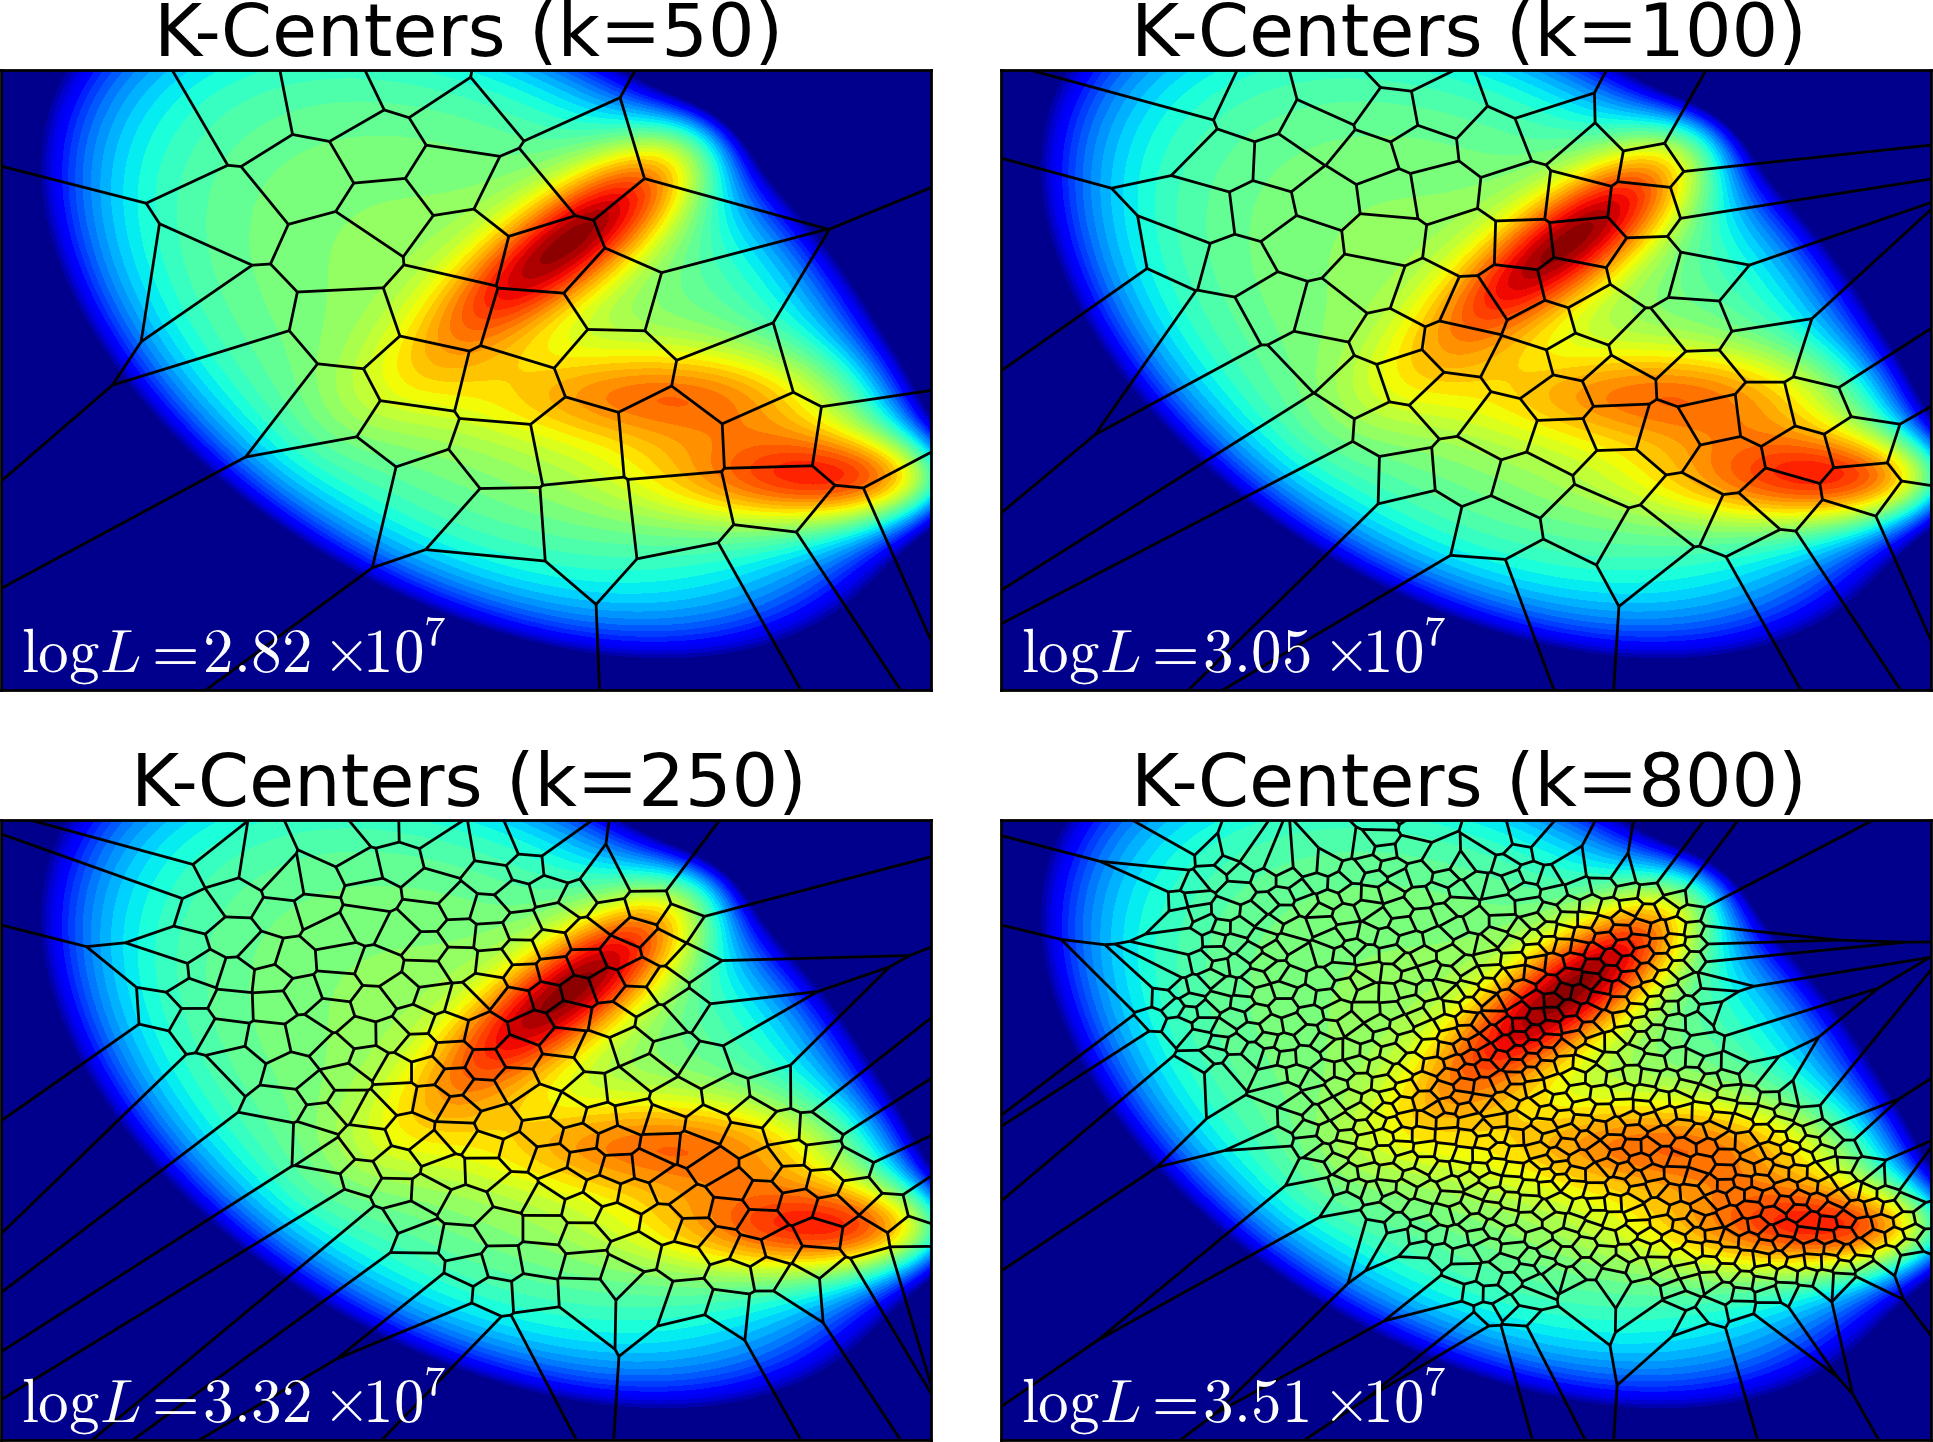
\includegraphics[width=5in]{figs/kcent_vors.png}
\caption{For K-Centers models, we observed a rapid increase in likelihood followed by a plateau. For models built with too few states, the states within the metastable wells are too large. By increasing the number of states, the resolution in increased, but using too many states leads to a model like the bottom right which is clearly over-fit and so has a non-optimal BIC despite having a higher likelihood.}
\end{figure*}

\begin{figure}
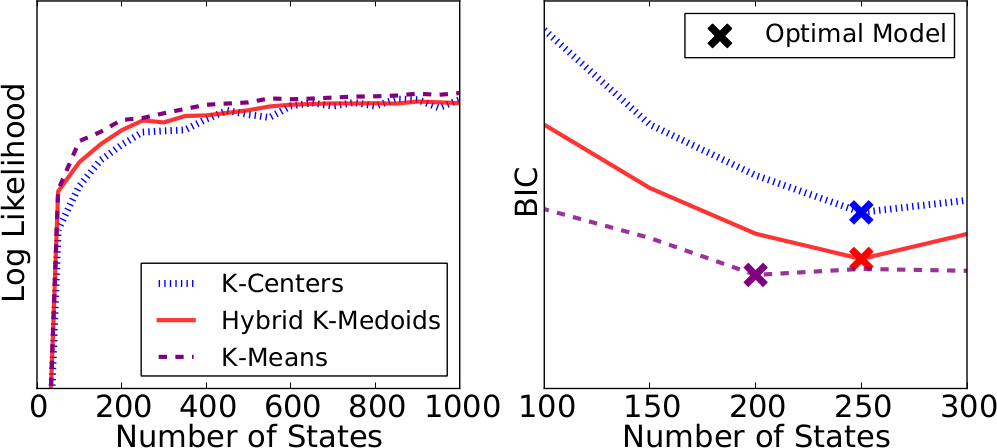
\includegraphics[width=3in]{figs/cluster_comp.png}
\caption{We also compared three clustering algorithms and used the likelihood function to determine which is best. The likelihood of the K-Means models was always larger than the other two. Additionally, the K-Means algorithm plateaued at a lower value of $k$, which corresponded to a minimum in the BIC curve at 200 states vs. the optimal models of 250 states in the K-Centers and Hybrid K-Medoids models.} \end{figure}

\begin{figure}
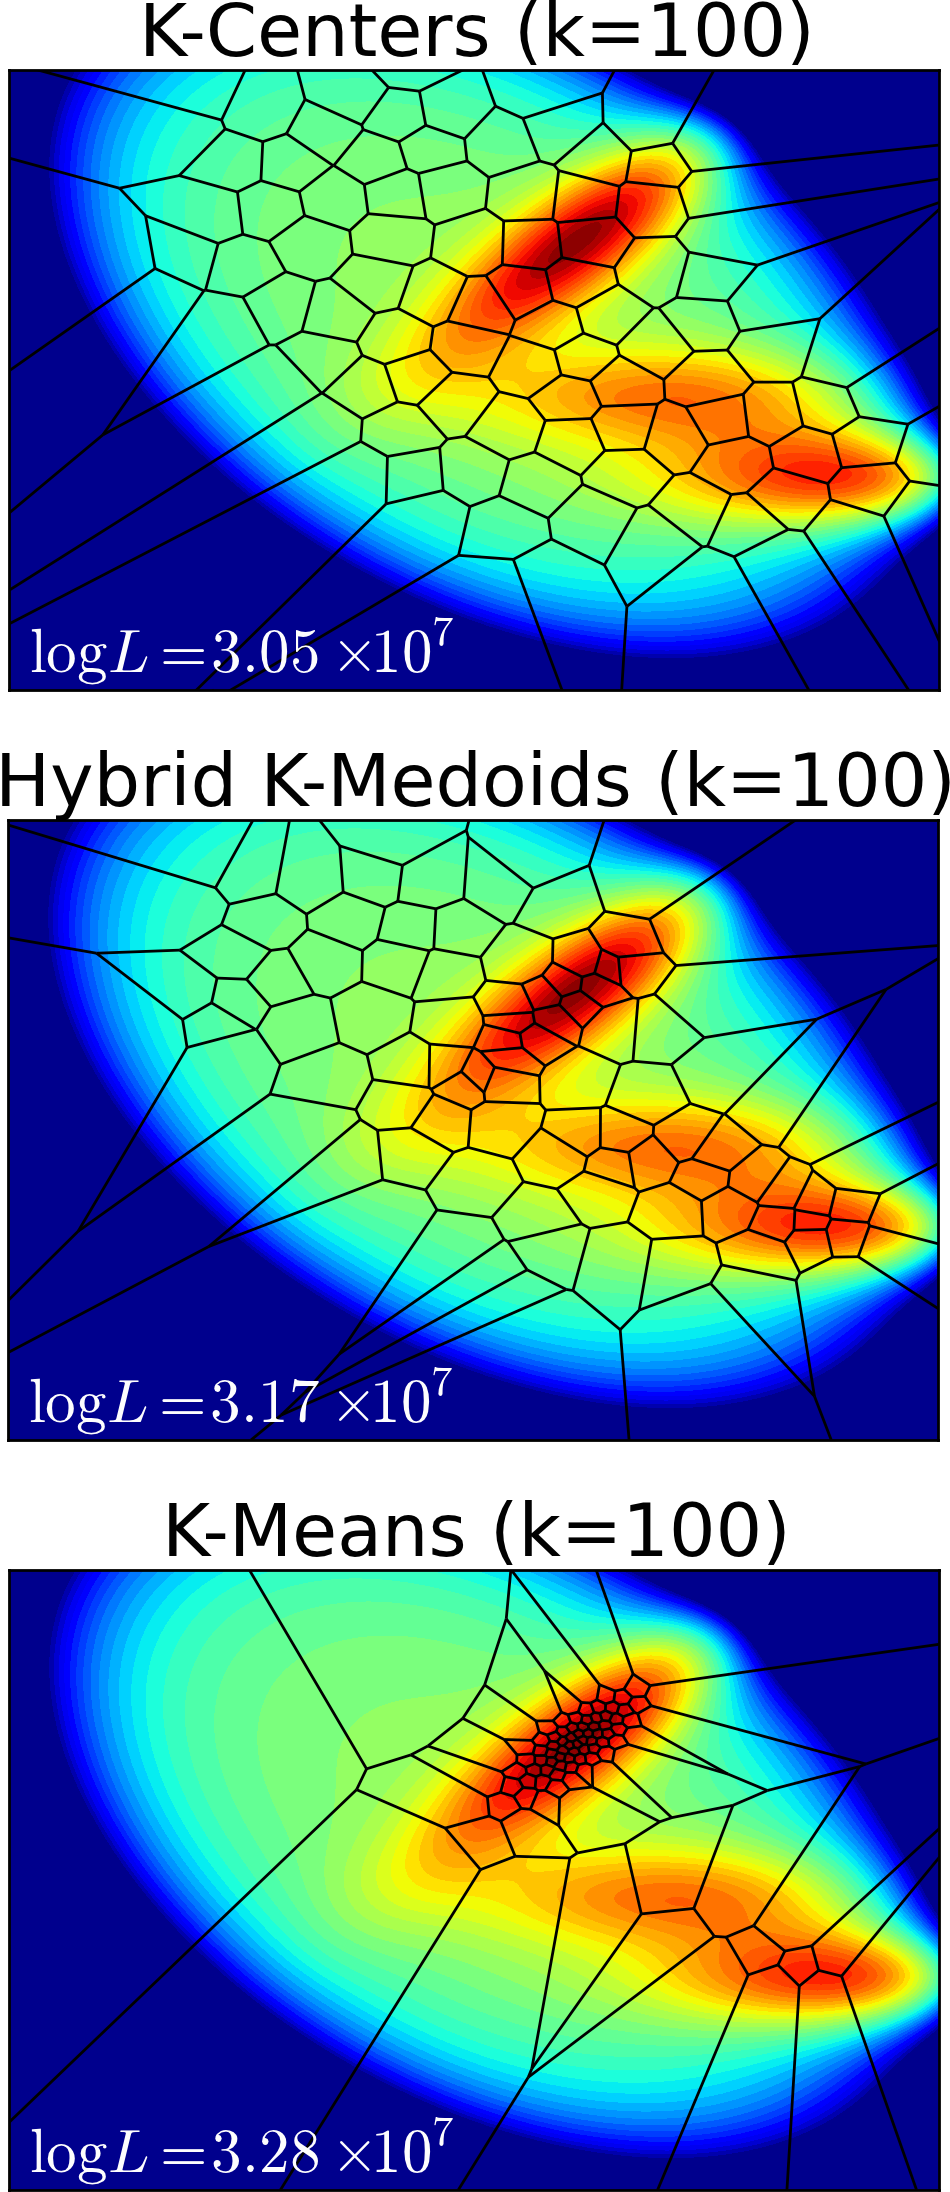
\includegraphics[width=2in]{figs/clust_vors.png}
\caption{The likelihoods (and BIC's) of the three clustering algorithms predicted that the K-Means algorithm is the better clustering algorithm. The result of K-Means is many states clustered into the highest density areas of the potential. The Hybrid K-Medoids ends up somewhere in between the K-Centers model and the K-Means model. This is likely due to the implementation being an approximate algorithm that requires more iterations to converge to the best state decomposition.}
\end{figure}
\bibliography{bibliography}
\end{document}
